\documentclass[11pt]{article}
\usepackage[utf8]{inputenc}
\usepackage{graphicx}
\usepackage{geometry}
\usepackage[table]{xcolor}
\usepackage{titlesec}
\usepackage{fancyhdr}
\usepackage{tocloft}
\usepackage{float}
\usepackage{ulem} 
\usepackage{tcolorbox}
\usepackage{tabularx}
\usepackage{longtable}
\usepackage{array}
\usepackage{booktabs}
\usepackage{listings}


\usepackage[colorlinks=true, linkcolor=black, urlcolor=black, citecolor=black]{hyperref}

\definecolor{myblue}{HTML}{2C56C9}
\definecolor{myline}{HTML}{253555}
\definecolor{sqlkeyword}{HTML}{0000FF}
\definecolor{sqlstring}{HTML}{008000}
\definecolor{sqlcomment}{HTML}{808080}


\lstdefinestyle{sqlstyle}{
    language=SQL,
    basicstyle=\ttfamily\small,
    keywordstyle=\color{sqlkeyword}\bfseries,
    stringstyle=\color{sqlstring},
    commentstyle=\color{sqlcomment}\itshape,
    numberstyle=\tiny\color{gray},
    breaklines=true,
    breakatwhitespace=true,
    showstringspaces=false,
    frame=none,
    numbers=none,
    tabsize=2,
    captionpos=b,
    morekeywords={GENERATED, ALWAYS, IDENTITY, PRIMARY, KEY, UNIQUE, NOT, NULL, CONSTRAINT, REFERENCES, CASCADE, CHECK, TRIGGER, FUNCTION, RETURNS, BEGIN, END, IF, THEN, ELSE, DECLARE, INTEGER, VARCHAR, TEXT, DATE, BOOLEAN}
}


\geometry{margin=2.5cm}

\setlength{\headheight}{15.4pt}
\addtolength{\topmargin}{-3.4pt}


\titleformat{\section}
{\color{myblue}\normalfont\Large\bfseries}
{\thesection}{1em}{}

\fancypagestyle{normal}{
    \fancyhf{}
    \fancyhead[L]{\textcolor{myblue}{Corsi di Studi in Informatica}}
    \fancyhead[R]{\textcolor{myblue}{00BD58}}
    \fancyfoot[L]{\textcolor{myblue}{UninaFoodLab}}
    \fancyfoot[C]{\thepage}
    \fancyfoot[R]{\textcolor{myblue}{2025/2026}}
    \renewcommand{\headrulewidth}{0.4pt}
    \renewcommand{\footrulewidth}{0.4pt}
    \renewcommand{\headrule}{\color{myline}\hrule height 0.4pt \vspace{3pt}}
    \renewcommand{\footrule}{\color{myline}\hrule height 0.4pt \vspace{3pt}}
}

\fancypagestyle{firstpage}{
    \fancyhf{}
    \fancyfoot[L]{\textcolor{myblue}{UninaFoodLab}}
    \fancyfoot[C]{\thepage}
    \fancyfoot[R]{\textcolor{myblue}{2025/2026}}
    \renewcommand{\headrulewidth}{0pt}
    \renewcommand{\footrulewidth}{0.4pt}
    \renewcommand{\footrule}{\color{myline}\hrule height 0.4pt \vspace{3pt}}
}

\renewcommand{\contentsname}{Indice}
\renewcommand{\cftsecfont}{\color{myblue}\bfseries}
\renewcommand{\cftsecpagefont}{\color{black}}
\renewcommand{\cftsubsecfont}{\color{black}}

\begin{document}



\thispagestyle{firstpage}


\begin{center}
    
\includegraphics[width=0.3\textwidth]{latex/immagini/uni_logo.png} 
    \vspace{0.5cm}

    {\large \textbf{Corso di Laurea in Informatica - Università degli Studi di Napoli Federico II}}\\
    {\large \textbf{A.A. 2025/2026}}\\[1cm]
    \vspace{1cm}

    {\Huge \color{myblue} \textbf{UninaFoodLab}}\\[2cm]

    \begin{flushleft}
    \centering
    {\large
    \textbf{Calone Francesco N86005555}\\
    \vspace{0.2cm}
    \textbf{D'Angelo Mario N86005477}\\
    }
    
    \vspace{0.2cm}
    {\small Codice gruppo: \textbf{OOBD39}}\\
    \vspace{0.8cm} 

    {\small Insegnamento di Basi di Dati I}
    \end{flushleft}
\end{center}


\newpage

\pagestyle{normal}

\tableofcontents
\thispagestyle{normal}

\section{Introduzione}
\subsection{Descrizione del progetto}
Il seguente progetto, denominato UninaFoodLab, nasce con l'obiettivo di progettare e implementare un sistema informativo per la gestione di corsi di cucina tematici. Il sistema si propone di supportare gli chef nella creazione e 
gestione di corsi articolati in sessioni teoriche e pratiche, facilitando al contempo l’iscrizione e la partecipazione degli utenti. \\
La documentazione che segue illustra in dettaglio tutte le fasi della progettazione, analizzando le scelte architetturali, i modelli concettuali e logici, e le soluzioni tecniche adottate per garantire la correttezza, la coerenza e l'efficienza del sistema.

\subsection{Analisi dei Requisiti rilenvanti per il Database}

I seguenti requisiti funzionali sono stati analizzati ai fini della progettazione della base di dati. Essi definiscono le informazioni da memorizzare e le relazioni tra le entità del sistema.

\begin{enumerate}
    \item Registrazione e autenticazione degli utenti.
    \begin{itemize}
        \item Gli utenti devono poter creare un account con email e password.
        \item Gli utenti devono poter effettuare il login.
    \end{itemize}

    \item Gestione dei profili utente.
    \begin{itemize}
        \item Gli utenti devono poter visualizzare e modificare le proprie informazioni personali.
        \item Gli utenti devono poter visualizzare i propri corsi.
        \item Gli utenti devono poter visualizzare i propri dati di pagamento.
        \item Gli utenti devono poter visualizzare le proprie sessioni pratiche.
    \end{itemize}

    \item Creazione e gestione dei corsi da parte degli chef.
    \begin{itemize}
        \item Gli chef devono poter creare nuovi corsi.
        \item Gli chef devono poter definire le sessioni teoriche e pratiche.
        \item Gli chef devono poter modificare.
        \item Gli chef possono aggiungere delle ricette alle sessioni pratiche.
        \item Gli chef devono poter visualizzare il numero di ingredienti necessari per la sessione pratica
        \item Gli chef devono poter visualizzare il loro report di guadagno e attività.
    \end{itemize}

    \item Iscrizione ai corsi da parte degli utenti.
    \begin{itemize}
        \item Gli utenti devono poter consultare l’elenco dei corsi disponibili.
        \item Gli utenti devono poter iscriversi a un corso.
        \item Gli utenti devono dare conferma per la partecipazione alle sessioni pratiche.
    \end{itemize}

    \item Gestione delle presenze e dei pagamenti.
    \begin{itemize}
        \item Gli chef devono poter registrare la presenza alle sessioni.
        \item Il sistema deve gestire i pagamenti degli utenti.
        \item Gli utenti devono poter vedere le proprie carte di credito.
    \end{itemize}
\end{enumerate}



\section{progettazione concettuale}
\subsection{Introduzione}
Il modello concettuale rappresenta la struttura logica del database, definendo le entità, gli attributi e le relazioni tra di esse. In questa fase, si è proceduto a identificare le principali entità del sistema e a stabilire le relazioni che le collegano, garantendo così una visione chiara e coerente delle informazioni da gestire.
\subsection{UML non ristrutturato}
\begin{figure}[H]
    \noindent\makebox[\linewidth]{%
        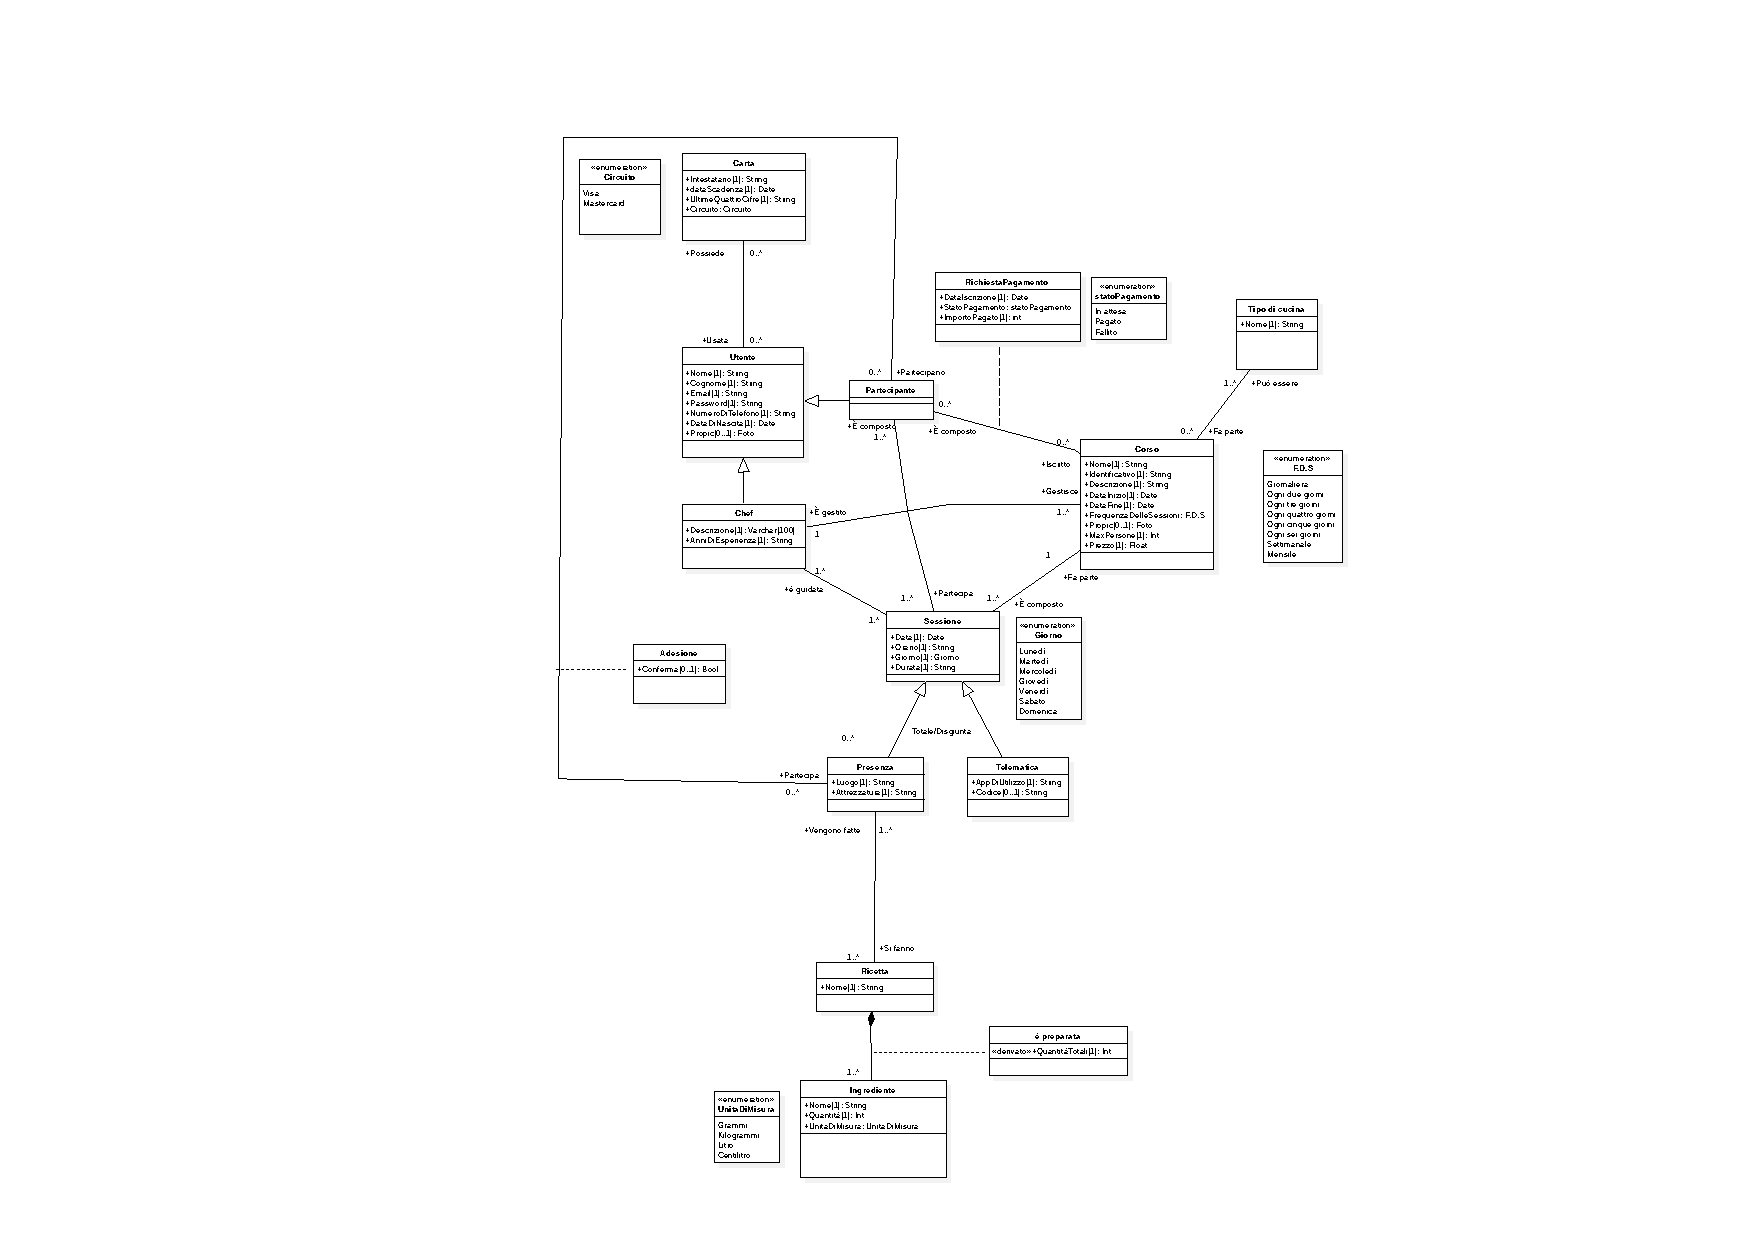
\includegraphics[height=0.9\textheight,width=2\textwidth]{latex/immagini/uml_non_ristrutturato.pdf}
    }
    \caption{Diagramma UML del sistema}
\end{figure}
\subsubsection{Entità principali}
Le entità principali identificate nel sistema sono:
\begin{itemize}
    \item \textbf{Utente}: L’utente rappresenta il soggetto fruitore del sistema, che può iscriversi ai corsi e partecipare alle sessioni. I principali attributi includono nome, cognome, email, password, telefono, data di nascita e una foto di profilo. Ogni utente può essere associato a una o più carte di pagamento e può diventare partecipante a diversi corsi.
    \item \textbf{Chef}: Lo chef è un utente con il ruolo specifico di organizzare corsi. Ogni chef dispone di una descrizione e di un numero di anni di esperienza. Un chef può gestire più corsi, ma ogni corso è gestito da un solo chef.
    \item \textbf{Corso}: Il corso è l'entità centrale del sistema e rappresenta una proposta didattica su un tema gastronomico specifico. Contiene attributi quali nome, descrizione, identificativo, data di inizio/fine, frequenza delle sessioni, prezzo, immagine di copertina e tipo di cucina (modellato come enumerazione). Ogni corso è composto da più sessioni e prevede una relazione molti-a-molti con i partecipanti.
    \item \textbf{Sessione}: Ogni corso è articolato in una o più sessioni, ciascuna delle quali ha una data, un orario, un insieme di giorni della settimana in cui si svolge, e una durata. Le sessioni sono specializzate in due sottotipi mutuamente esclusivi:
    \begin{itemize}
        \item \textbf{Presenza}: Con attributi come luogo e attrezzature richieste.
        \item \textbf{Telematica}: Con attributi relativi all'app utilizzata e al codice di accesso.
    \end{itemize}
    \item \textbf{Partecipante e Adesione}: La partecipazione ai corsi è modellata tramite l’entità Partecipante, che collega utenti e corsi. La partecipazione a sessioni pratiche richiede un’adesione esplicita, rappresentata dall'entità Adesione, che contiene un attributo booleano di conferma.
    \item \textbf{Ricetta e Ingredientemento}: Ogni sessione pratica può includere la preparazione di una o più ricette. Ogni ricetta è composta da uno o più ingredienti, ciascuno dei quali ha un nome, una quantità e un'unità di misura (enumerata). La relazione tra Ricetta e Ingrediente è associativa e include l'attributo QuantitàTotale, utile per calcolare la quantità necessaria in base alle adesioni.
    \item \textbf{Carta e RichiestaPagamento}: Gli utenti possono associare al proprio profilo una o più carte di pagamento, appartenenti a un circuito specificato tramite enumerazione (Visa, Mastercard). Le richieste di pagamento sono entità separate, con data, stato (in attesa, pagato, fallito) e importo.
\end{itemize}
\subsubsection{Gerarchie e generalizzazioni}
Nel modello concettuale, sono state identificate le seguenti gerarchie e generalizzazioni:
\begin{itemize}
    \item \textbf{Sessione}: Le sessioni sono suddivise in due sottotipi: \textit{Presenza} e \textit{Telematica}. Questa specializzazione consente di gestire le specificità di ciascun tipo di sessione, come il luogo e le attrezzature per le sessioni in presenza, e l'app utilizzata e il codice di accesso per quelle telematiche.
    \item \textbf{Utente}: L'entità Utente può essere specializzata in due sottotipi: \textit{Partecipante} e \textit{Chef}. Questa distinzione permette di gestire le diverse funzionalità e attributi associati a ciascun ruolo nel sistema.
\end{itemize}
Entrambe le specializzazioni sono totali e disgiunte, di conseguenza ogni istanza di Sessione sia esclusivamente di uno dei due tipi e che ogni Utente sia o un Partecipante o uno Chef, ma non entrambi contemporaneamente.
\subsubsection{Relazioni tra le entità}
Le relazioni tra le entità sono state definite come segue:
\begin{itemize}
    \item \textbf{Utente - Partecipante}: Un utente può essere un partecipante a più corsi, e ogni corso può avere più partecipanti. Questa relazione è molti-a-molti.
    \item \textbf{Chef - Corso}: Ogni chef può gestire più corsi, ma ogni corso è associato a un solo chef. Questa relazione è uno-a-molti.
    \item \textbf{Corso - Sessione}: Un corso può avere più sessioni, ma ogni sessione appartiene a un solo corso. Questa relazione è uno-a-molti.
    \item \textbf{Sessione - Partecipante}: Ogni partecipante può aderire a più sessioni pratiche, e ogni sessione può avere più partecipanti. Questa relazione è molti-a-molti, mediata dall'entità Adesione.
    \item \textbf{Corso - Ricetta}: Ogni corso può includere più ricette, e ogni ricetta può essere associata a più corsi. Questa relazione è molti-a-molti.
    \item \textbf{Ricetta - Ingrediente}: Ogni ricetta può includere più ingredienti, e ogni ingrediente può essere utilizzato in più ricette. Questa relazione è molti-a-molti, mediata dall'attributo QuantitàTotale.
    \item \textbf{Utente - Carta}: Un utente può avere più carte di pagamento associate al proprio profilo. Questa relazione è uno-a-molti.
    \item \textbf{Ricetta - Ingrediente}: Ogni ricetta può essere associata a più ingredienti, e ogni ingrediente può essere utilizzato in più ricette. Questa relazione è una composizione, mediata dall'attributo QuantitàTotale.
\end{itemize}
\subsubsection{Motivazione delle scelte progettuali}
Le scelte progettuali sono state guidate dalla necessità di garantire una rappresentazione chiara e coerente delle informazioni, facilitando la gestione dei corsi, delle sessioni e delle partecipazioni. La specializzazione delle sessioni in Presenza e Telematica consente di gestire le specificità di ciascun tipo di sessione, mentre la distinzione tra Partecipante e Chef permette di differenziare i ruoli degli utenti nel sistema. Inoltre, l'uso di relazioni molti-a-molti per gestire le adesioni alle sessioni pratiche e le associazioni tra ricette e ingredienti garantisce flessibilità e scalabilità nel modello.



\section{Architettura del Progetto}

L'architettura del progetto UninaFoodLab è stata progettata per garantire una chiara separazione dei compiti e una facile manutenibilità. La struttura delle directory riflette i principali livelli logici dell'applicazione, secondo il pattern MVC e le best practice di progettazione.

Le principali suddivisioni sono:
\begin{itemize}
    \item \textbf{Boundary}: contiene le classi responsabili dell'interfaccia grafica e dell'interazione con l'utente, realizzate tramite JavaFX e FXML.
    \item \textbf{Controller}: gestisce la logica applicativa e il flusso degli eventi tra la GUI e i dati.
    \item \textbf{Entity}: suddivisa ulteriormente in \textit{DAO} (Data Access Object) e \textit{DTO} (Data Transfer Object). I DAO si occupano della persistenza e dell'accesso ai dati, mentre i DTO rappresentano le strutture dati scambiate tra i vari livelli.
    \item \textbf{JDBC}: contiene le classi e le utility per la connessione e la gestione del database PostgreSQL.
    \item \textbf{Utils}: raccoglie le classi di supporto e gli strumenti riutilizzabili all'interno del progetto.
\end{itemize}
Questa organizzazione favorisce la modularità e la scalabilità del sistema, permettendo di isolare le responsabilità e facilitare l'estensione futura. Ogni componente interagisce con gli altri tramite interfacce ben definite, riducendo le dipendenze e migliorando la qualità del codice.

La scelta di suddividere le entity in DAO e DTO consente di gestire in modo efficiente sia la persistenza che il trasferimento dei dati, mentre la presenza di una directory dedicata alle utility semplifica la gestione delle funzionalità trasversali.

\subsection{Struttura delle Directory}
La struttura delle directory del progetto è organizzata come segue:
\begin{itemize}
    \item \textbf{src/main/java}: contiene il codice sorgente dell'applicazione.
    \item \textbf{src/main/resources}: contiene le risorse dell'applicazione, come file FXML e immagini.
    \item \textbf{src/test/java}: contiene i test automatizzati.
\end{itemize}


\section{Definizioni SQL}

\subsection{Introduzione}

In questo capitolo viene presentata l'implementazione pratica del database UninaFoodLab attraverso la definizione completa del codice SQL sviluppato in PostgreSQL. La sezione fornisce una panoramica dettagliata di tutti gli elementi che compongono il database, dalla creazione delle tabelle all'implementazione delle funzioni.


\subsection{Definizione degli enumerati}

Gli enumerati sono tipi di dato definiti dall’utente che permettono di vincolare il valore di un attributo a un insieme finito di possibilità predefinite. Nel database UninaFoodLab vengono utilizzati per rappresentare domini chiusi come circuiti di carte, stati di pagamento, frequenza delle sessioni, giorni della settimana e unità di misura degli ingredienti. Questo garantisce coerenza e integrità dei dati, semplificando la gestione delle regole applicative.

\noindent\rule{\textwidth}{0.4pt}
\begin{lstlisting}[language=SQL, style=sqlstyle, literate={à}{{\`a}}1 {è}{{\`e}}1 {é}{{\'e}}1 {ì}{{\`i}}1 {ò}{{\`o}}1 {ù}{{\`u}}1]
CREATE TYPE Circuito AS ENUM ('Visa', 'Mastercard');

CREATE TYPE StatoPagamento AS ENUM ('In attesa', 'Pagato', 'Fallito');

CREATE TYPE FDS AS ENUM (
  'Giornaliera',
  'Ogni due giorni',
  'Ogni tre giorni',
  'Ogni quattro giorni',
  'Ogni cinque giorni',
  'Ogni sei giorni',
  'Settimanale',
  'Mensile'
);

CREATE TYPE Giorno AS ENUM (
  'Lunedì',
  'Martedì',
  'Mercoledì',
  'Giovedì',
  'Venerdì',
  'Sabato',
  'Domenica'
);

CREATE TYPE UnitaDiMisura AS ENUM ('Grammi', 'Kilogrammi', 'Litro', 'Centilitro');
\end{lstlisting}
\noindent\rule{\textwidth}{0.4pt}

\subsection{Definizione delle Tabelle}


\subsubsection{Tabella Partecipante}

La tabella \texttt{Partecipante} rappresenta gli utenti che si iscrivono e partecipano ai corsi di cucina. Ogni partecipante ha un identificativo univoco generato automaticamente e deve fornire informazioni personali essenziali per la registrazione.

\noindent\rule{\textwidth}{0.4pt}
\begin{lstlisting}[language=SQL, style=sqlstyle]
CREATE TABLE Partecipante (
    IdPartecipante INT GENERATED ALWAYS AS IDENTITY PRIMARY KEY,
    Nome VARCHAR(50) NOT NULL,
    Cognome VARCHAR(50) NOT NULL,
    Email VARCHAR(100) UNIQUE NOT NULL,
    Password VARCHAR(100) NOT NULL,
    DataDiNascita DATE NOT NULL,
    Propic TEXT
);
\end{lstlisting}
\noindent\rule{\textwidth}{0.4pt}

\textbf{Scelte progettuali:}
\begin{itemize}
    \item \textbf{IdPartecipante}: Chiave primaria auto-incrementale utilizzando \texttt{GENERATED ALWAYS AS IDENTITY} per garantire unicità automatica
    \item \textbf{Email}: Constraint \texttt{UNIQUE} per evitare registrazioni duplicate
    \item \textbf{Password}: Campo di lunghezza fissa per supportare hash di password sicure
    \item \textbf{Propic}: Campo \texttt{TEXT} per supportare URL di immagini o dati base64
\end{itemize}

\subsubsection{Tabella Carta}

La tabella \texttt{Carta} memorizza le carte di pagamento associate agli utenti. Ogni carta ha un identificativo univoco, intestatario, data di scadenza, ultime quattro cifre e circuito di appartenenza.

\noindent\rule{\textwidth}{0.4pt}
\begin{lstlisting}[language=SQL, style=sqlstyle]
CREATE TABLE Carta (
    IdCarta INT GENERATED ALWAYS AS IDENTITY PRIMARY KEY,
    Intestatario VARCHAR(100) NOT NULL,
    DataScadenza DATE NOT NULL,
    UltimeQuattroCifre CHAR(4) NOT NULL,
    Circuito VARCHAR(50) NOT NULL
);
\end{lstlisting}
\noindent\rule{\textwidth}{0.4pt}

\textbf{Scelte progettuali:}
\begin{itemize}
    \item \textbf{IdCarta}: Chiave primaria auto-incrementale
    \item \textbf{Intestatario, DataScadenza, UltimeQuattroCifre, Circuito}: Attributi essenziali per identificare una carta
    \item \textbf{Circuito}: Vincolato tramite tipo enumerato per coerenza
\end{itemize}

\subsubsection{Tabella Possiede}

La tabella \texttt{Possiede} rappresenta la relazione molti-a-molti tra partecipanti e carte, indicando quali carte sono possedute da ciascun partecipante.

\noindent\rule{\textwidth}{0.4pt}
\begin{lstlisting}[language=SQL, style=sqlstyle]
CREATE TABLE Possiede (
    IdPartecipante INT,
    IdCarta INT,
    PRIMARY KEY (IdPartecipante, IdCarta),
    FOREIGN KEY (IdPartecipante) REFERENCES Partecipante(IdPartecipante),
    FOREIGN KEY (IdCarta) REFERENCES Carta(IdCarta) on delete cascade 
);
\end{lstlisting}
\noindent\rule{\textwidth}{0.4pt}

\textbf{Scelte progettuali:}
\begin{itemize}
    \item \textbf{Chiave primaria composta}: (IdPartecipante, IdCarta) per garantire unicità della relazione
    \item \textbf{Vincoli di integrità}: Foreign key verso \texttt{Partecipante} e \texttt{Carta}
    \item \textbf{Cascata}: Eliminazione a cascata delle carte
\end{itemize}

\subsubsection{Tabella Corso}

La tabella \texttt{Corso} rappresenta i corsi di cucina offerti, con informazioni su nome, descrizione, periodo, frequenza, prezzo, chef responsabile e limiti di partecipazione.

\noindent\rule{\textwidth}{0.4pt}
\begin{lstlisting}[language=SQL, style=sqlstyle]
CREATE TABLE Corso (
    IdCorso INT GENERATED ALWAYS AS IDENTITY PRIMARY KEY,
    Nome VARCHAR(100) NOT NULL,
    Descrizione VARCHAR(60) NOT NULL,
    DataInizio DATE NOT NULL,
    DataFine DATE NOT NULL,
    FrequenzaDelleSessioni VARCHAR(100) NOT NULL,
    Propic TEXT,
    MaxPersone INT CHECK (MaxPersone > 0),
    Prezzo DECIMAL(10, 2) CHECK (Prezzo >= 0),
    IdChef INT NOT NULL,
    FOREIGN KEY (IdChef) REFERENCES Chef(IdChef)
);
\end{lstlisting}
\noindent\rule{\textwidth}{0.4pt}

\textbf{Scelte progettuali:}
\begin{itemize}
    \item \textbf{IdCorso}: Chiave primaria auto-incrementale
    \item \textbf{MaxPersone, Prezzo}: Vincoli di validità sui valori
    \item \textbf{IdChef}: Foreign key verso chef responsabile
    \item \textbf{FrequenzaDelleSessioni}: Vincolata tramite tipo enumerato
\end{itemize}

\subsubsection{Tabella RichiestaPagamento}

La tabella \texttt{RichiestaPagamento} registra le richieste di pagamento per i corsi, associando ogni richiesta a un partecipante e a un corso specifico, con informazioni su importo, stato e data.

\noindent\rule{\textwidth}{0.4pt}
\begin{lstlisting}[language=SQL, style=sqlstyle]
CREATE TABLE RichiestaPagamento (
    DataRichiesta TIMESTAMP NOT NULL,
    StatoPagamento VARCHAR(50) NOT NULL,
    ImportoPagato DECIMAL(10, 2) CHECK (ImportoPagato >= 0),
    IdCorso INT,
    IdPartecipante INT,
    PRIMARY KEY (DataRichiesta, IdCorso, IdPartecipante),
    FOREIGN KEY (IdCorso) REFERENCES Corso(IdCorso),
    FOREIGN KEY (IdPartecipante) REFERENCES Partecipante(IdPartecipante)
);
\end{lstlisting}
\noindent\rule{\textwidth}{0.4pt}

\textbf{Scelte progettuali:}
\begin{itemize}
    \item \textbf{Chiave primaria composta}: (DataRichiesta, IdCorso, IdPartecipante)
    \item \textbf{ImportoPagato}: Vincolo di non negatività
    \item \textbf{StatoPagamento}: Vincolato tramite tipo enumerato
    \item \textbf{Foreign key}: Collegamento a corso e partecipante
\end{itemize}

\subsubsection{Tabella TipoDiCucina}

La tabella \texttt{TipoDiCucina} elenca le tipologie di cucina disponibili, ciascuna con un identificativo univoco e un nome.

\noindent\rule{\textwidth}{0.4pt}
\begin{lstlisting}[language=SQL, style=sqlstyle]
CREATE TABLE TipoDiCucina (
    IDTipoCucina INT GENERATED ALWAYS AS IDENTITY PRIMARY KEY,
    Nome VARCHAR(50) NOT NULL UNIQUE
);
\end{lstlisting}
\noindent\rule{\textwidth}{0.4pt}

\textbf{Scelte progettuali:}
\begin{itemize}
    \item \textbf{IDTipoCucina}: Chiave primaria auto-incrementale
    \item \textbf{Nome}: Unicità per evitare duplicati
\end{itemize}

\subsubsection{Tabella TipoDiCucina\_Corso}

La tabella \texttt{TipoDiCucina\_Corso} rappresenta l'associazione tra corsi e tipologie di cucina, permettendo di collegare più tipi di cucina a ciascun corso (fino a un massimo di due).

\noindent\rule{\textwidth}{0.4pt}
\begin{lstlisting}[language=SQL, style=sqlstyle]
CREATE TABLE TipoDiCucina_Corso (
    IDTipoCucina INT,
    IDCorso INT,
    PRIMARY KEY (IDTipoCucina, IDCorso),
    FOREIGN KEY (IDTipoCucina) REFERENCES TipoDiCucina(IDTipoCucina),
    FOREIGN KEY (IDCorso) REFERENCES Corso(IdCorso)
);
\end{lstlisting}
\noindent\rule{\textwidth}{0.4pt}

\textbf{Scelte progettuali:}
\begin{itemize}
    \item \textbf{Chiave primaria composta}: (IDTipoCucina, IDCorso)
    \item \textbf{Foreign key}: Collegamento a tipo di cucina e corso
    \item \textbf{Vincolo applicativo}: Massimo due tipi di cucina per corso (gestito da trigger)
\end{itemize}

\subsubsection{Tabella Chef}

La tabella \texttt{Chef} contiene le informazioni sugli chef che tengono i corsi. Oltre ai dati anagrafici, include una descrizione e gli anni di esperienza.

\noindent\rule{\textwidth}{0.4pt}
\begin{lstlisting}[language=SQL, style=sqlstyle]
CREATE TABLE Chef (
    IdChef INT GENERATED ALWAYS AS IDENTITY PRIMARY KEY,
    Nome VARCHAR(50) NOT NULL,
    Cognome VARCHAR(50) NOT NULL,
    Email VARCHAR(100) UNIQUE NOT NULL,
    Password VARCHAR(100) NOT NULL,
    DataDiNascita DATE NOT NULL,
    Descrizione VARCHAR(60),
    Propic TEXT,
    AnniDiEsperienza INT CHECK (AnniDiEsperienza >= 0)
);
\end{lstlisting}
\noindent\rule{\textwidth}{0.4pt}

\textbf{Scelte progettuali:}
\begin{itemize}
    \item \textbf{IdChef}: Chiave primaria auto-incrementale
    \item \textbf{Email}: Unicità per evitare duplicati
    \item \textbf{AnniDiEsperienza}: Vincolo di non negatività
    \item \textbf{Propic}: Supporto per immagine profilo
\end{itemize}

\subsubsection{Tabella Sessione\_Presenza}

La tabella \texttt{Sessione\_Presenza} descrive le sessioni in presenza dei corsi, con dettagli su luogo, data, orario, durata e chef responsabile.

\noindent\rule{\textwidth}{0.4pt}
\begin{lstlisting}[language=SQL, style=sqlstyle]
CREATE TABLE Sessione_Presenza (
    IdSessionePresenza INT GENERATED ALWAYS AS IDENTITY PRIMARY KEY,
    Giorno VARCHAR(20) NOT NULL,
    Data DATE NOT NULL,
    Orario TIME NOT NULL,
    Durata INTERVAL NOT NULL,
    Citta VARCHAR(50) NOT NULL,
    Via VARCHAR(100) NOT NULL,
    Cap CHAR(5) NOT NULL,
    Descrizione VARCHAR(60) NOT NULL,
    IdCorso INT,
    IdChef INT,
    FOREIGN KEY (IdCorso) REFERENCES Corso(IdCorso),
    FOREIGN KEY (IdChef) REFERENCES Chef(IdChef)
);
\end{lstlisting}
\noindent\rule{\textwidth}{0.4pt}

\textbf{Scelte progettuali:}
\begin{itemize}
    \item \textbf{IdSessionePresenza}: Chiave primaria auto-incrementale
    \item \textbf{Attributi luogo}: Città, via, cap per identificare la sede
    \item \textbf{Foreign key}: Collegamento a corso e chef
\end{itemize}

\subsubsection{Tabella Adesione\_SessionePresenza}

La tabella \texttt{Adesione\_SessionePresenza} registra l'adesione dei partecipanti alle sessioni in presenza, con conferma di partecipazione.

\noindent\rule{\textwidth}{0.4pt}
\begin{lstlisting}[language=SQL, style=sqlstyle]
CREATE TABLE Adesione_SessionePresenza (
    Conferma BOOLEAN,
    IdSessionePresenza INT,
    IdPartecipante INT,
    PRIMARY KEY (IdSessionePresenza, IdPartecipante),
    FOREIGN KEY (IdSessionePresenza) REFERENCES Sessione_Presenza(IdSessionePresenza),
    FOREIGN KEY (IdPartecipante) REFERENCES Partecipante(IdPartecipante)
);
\end{lstlisting}
\noindent\rule{\textwidth}{0.4pt}

\textbf{Scelte progettuali:}
\begin{itemize}
    \item \textbf{Chiave primaria composta}: (IdSessionePresenza, IdPartecipante)
    \item \textbf{Conferma}: Indica la presenza effettiva
    \item \textbf{Foreign key}: Collegamento a sessione presenza e partecipante
\end{itemize}

\subsubsection{Tabella Sessione\_Telematica}

La tabella \texttt{Sessione\_Telematica} descrive le sessioni online dei corsi, con dettagli su applicazione, codice chiamata, data, orario, durata e chef responsabile.

\noindent\rule{\textwidth}{0.4pt}
\begin{lstlisting}[language=SQL, style=sqlstyle]
CREATE TABLE Sessione_Telematica (
    IdSessioneTelematica INT GENERATED ALWAYS AS IDENTITY PRIMARY KEY,
    Applicazione VARCHAR(100) NOT NULL,
    CodiceChiamata VARCHAR(100) NOT NULL,
    Data DATE NOT NULL,
    Orario TIME NOT NULL,
    Durata INTERVAL NOT NULL,
    Giorno VARCHAR(20) NOT NULL,
    Descrizione VARCHAR(60) NOT NULL,
    IdCorso INT,
    IdChef INT,
    FOREIGN KEY (IdCorso) REFERENCES Corso(IdCorso),
    FOREIGN KEY (IdChef) REFERENCES Chef(IdChef)
);
\end{lstlisting}
\noindent\rule{\textwidth}{0.4pt}

\textbf{Scelte progettuali:}
\begin{itemize}
    \item \textbf{IdSessioneTelematica}: Chiave primaria auto-incrementale
    \item \textbf{Applicazione, CodiceChiamata}: Dettagli per l'accesso online
    \item \textbf{Foreign key}: Collegamento a corso e chef
\end{itemize}

\subsubsection{Tabella Partecipante\_SessioneTelematica}

La tabella \texttt{Partecipante\_SessioneTelematica} rappresenta la partecipazione dei partecipanti alle sessioni telematiche, associando ogni partecipante a una specifica sessione online.

\noindent\rule{\textwidth}{0.4pt}
\begin{lstlisting}[language=SQL, style=sqlstyle]
CREATE TABLE Partecipante_SessioneTelematica (
    IdPartecipante INT,
    IdSessioneTelematica INT,
    PRIMARY KEY (IdPartecipante, IdSessioneTelematica),
    FOREIGN KEY (IdPartecipante) REFERENCES Partecipante(IdPartecipante),
    FOREIGN KEY (IdSessioneTelematica) REFERENCES Sessione_Telematica(IdSessioneTelematica)
);
\end{lstlisting}
\noindent\rule{\textwidth}{0.4pt}

\textbf{Scelte progettuali:}
\begin{itemize}
    \item \textbf{Chiave primaria composta}: (IdPartecipante, IdSessioneTelematica)
    \item \textbf{Foreign key}: Collegamento a partecipante e sessione telematica
\end{itemize}

\subsubsection{Tabella Ricetta}

La tabella \texttt{Ricetta} contiene le ricette che possono essere preparate durante le sessioni dei corsi.

\noindent\rule{\textwidth}{0.4pt}
\begin{lstlisting}[language=SQL, style=sqlstyle]
CREATE TABLE Ricetta (
    IdRicetta INT GENERATED ALWAYS AS IDENTITY PRIMARY KEY,
    Nome VARCHAR(100) NOT NULL
);
\end{lstlisting}
\noindent\rule{\textwidth}{0.4pt}

\textbf{Scelte progettuali:}
\begin{itemize}
    \item \textbf{IdRicetta}: Chiave primaria auto-incrementale
    \item \textbf{Nome}: Nome della ricetta, obbligatorio
\end{itemize}

\subsubsection{Tabella Sessione\_Presenza\_Ricetta}

La tabella \texttt{Sessione\_Presenza\_Ricetta} associa le ricette alle sessioni in presenza, indicando quali ricette vengono preparate in ciascuna sessione.

\noindent\rule{\textwidth}{0.4pt}
\begin{lstlisting}[language=SQL, style=sqlstyle]
CREATE TABLE Sessione_Presenza_Ricetta (
    IdRicetta INT,
    IdSessionePresenza INT,
    PRIMARY KEY (IdRicetta, IdSessionePresenza),
    FOREIGN KEY (IdRicetta) REFERENCES Ricetta(IdRicetta),
    FOREIGN KEY (IdSessionePresenza) REFERENCES Sessione_Presenza(IdSessionePresenza)
);
\end{lstlisting}
\noindent\rule{\textwidth}{0.4pt}

\textbf{Scelte progettuali:}
\begin{itemize}
    \item \textbf{Chiave primaria composta}: (IdRicetta, IdSessionePresenza)
    \item \textbf{Foreign key}: Collegamento a ricetta e sessione presenza
\end{itemize}

\subsubsection{Tabella Ingrediente}

La tabella \texttt{Ingrediente} elenca tutti gli ingredienti disponibili, con nome e unità di misura.

\noindent\rule{\textwidth}{0.4pt}
\begin{lstlisting}[language=SQL, style=sqlstyle]
CREATE TABLE Ingrediente (
    IdIngrediente INT GENERATED ALWAYS AS IDENTITY PRIMARY KEY,
    Nome VARCHAR(100) NOT NULL,
    UnitaDiMisura VARCHAR(50) NOT NULL
);
\end{lstlisting}
\noindent\rule{\textwidth}{0.4pt}

\textbf{Scelte progettuali:}
\begin{itemize}
    \item \textbf{IdIngrediente}: Chiave primaria auto-incrementale
    \item \textbf{UnitaDiMisura}: Vincolata tramite tipo enumerato
\end{itemize}

\subsubsection{Tabella PreparazioneIngrediente}

La tabella \texttt{PreparazioneIngrediente} collega le ricette agli ingredienti necessari, specificando quantità totale e unitaria per ogni ingrediente in una ricetta.

\noindent\rule{\textwidth}{0.4pt}
\begin{lstlisting}[language=SQL, style=sqlstyle]
CREATE TABLE PreparazioneIngrediente (
    IdRicetta INT,
    IdIngrediente INT,
    QuantitaTotale DECIMAL(10,2) CHECK (QuantitaTotale >= 0),
    QuanititaUnitaria DECIMAL(10,2) NOT NULL CHECK (QuanititaUnitaria >= 0),
    PRIMARY KEY (IdRicetta, IdIngrediente),
    FOREIGN KEY (IdRicetta) REFERENCES Ricetta(IdRicetta),
    FOREIGN KEY (IdIngrediente) REFERENCES Ingrediente(IdIngrediente)
);
\end{lstlisting}
\noindent\rule{\textwidth}{0.4pt}

\textbf{Scelte progettuali:}
\begin{itemize}
    \item \textbf{Chiave primaria composta}: (IdRicetta, IdIngrediente)
    \item \textbf{QuantitaTotale, QuanititaUnitaria}: Vincoli di non negatività
    \item \textbf{Foreign key}: Collegamento a ricetta e ingrediente
\end{itemize}



\subsection{Definizione dei Trigger}

\setlength{\headheight}{17pt}

\subsubsection{Trigger: Unicità Email tra Chef e Partecipante}

Questo trigger garantisce che lo stesso indirizzo email non possa essere usato contemporaneamente da un Chef e da un Partecipante. La funzione viene richiamata sia sulle tabelle Chef che Partecipante, in inserimento e aggiornamento.

\noindent\rule{\textwidth}{0.4pt}
\begin{lstlisting}[language=SQL, style=sqlstyle, literate={à}{{\`a}}1 {è}{{\`e}}1 {é}{{\'e}}1 {ì}{{\`i}}1 {ò}{{\`o}}1 {ù}{{\`u}}1]
CREATE OR REPLACE FUNCTION verifica_unicita_email()
RETURNS TRIGGER AS $$
BEGIN
    IF TG_TABLE_NAME = 'chef' THEN
        IF EXISTS (SELECT 1 FROM partecipante WHERE email = NEW.email) THEN
            RAISE EXCEPTION 'Errore: L''email "%" è già utilizzata da un Partecipante.', NEW.email;
        END IF;
    ELSIF TG_TABLE_NAME = 'partecipante' THEN
        IF EXISTS (SELECT 1 FROM chef WHERE email = NEW.email) THEN
            RAISE EXCEPTION 'Errore: L''email "%" è già utilizzata da uno Chef.', NEW.email;
        END IF;
    END IF;
    RETURN NEW;
END;
$$ LANGUAGE plpgsql;

CREATE TRIGGER trg_verifica_email_partecipante
BEFORE INSERT OR UPDATE ON partecipante
FOR EACH ROW
EXECUTE FUNCTION verifica_unicita_email();

CREATE TRIGGER trg_verifica_email_chef
BEFORE INSERT OR UPDATE ON chef
FOR EACH ROW
EXECUTE FUNCTION verifica_unicita_email();
\end{lstlisting}
\noindent\rule{\textwidth}{0.4pt}

\textbf{Spiegazione:}
\begin{itemize}
    \item \texttt{IF TG\_TABLE\_NAME = 'chef'}: Se il trigger è attivato dalla tabella Chef, controlla che l'email inserita o aggiornata non sia già presente nella tabella \texttt{partecipante} (campo \texttt{email}).
    \item \texttt{IF TG\_TABLE\_NAME = 'partecipante'}: Se il trigger è attivato dalla tabella Partecipante, controlla che l'email inserita o aggiornata non sia già presente nella tabella \texttt{chef} (campo \texttt{email}).
    \item \texttt{IF EXISTS (SELECT 1 ...)}: In entrambi i casi, se trova una corrispondenza, solleva un'eccezione e blocca l'inserimento/aggiornamento.
    \item \texttt{RAISE EXCEPTION}: Genera un errore se l'email è già in uso nell'altra tabella.
    \item Il trigger si attiva prima dell'inserimento o aggiornamento di un record (\texttt{BEFORE INSERT OR UPDATE}) sia su Chef che su Partecipante, garantendo l'unicità trasversale dell'email tra le due tabelle.
\end{itemize}

\subsubsection{Trigger: Controllo Formato Email}

Questo trigger verifica che l'indirizzo email inserito per Chef e Partecipante sia formalmente valido, ovvero contenga una chiocciola (@) e almeno un punto dopo la chiocciola, garantendo la correttezza sintattica degli indirizzi email memorizzati nel sistema.

\noindent\rule{\textwidth}{0.4pt}
\begin{lstlisting}[language=SQL, style=sqlstyle, literate={à}{{\`a}}1 {è}{{\`e}}1 {é}{{\'e}}1 {ì}{{\`i}}1 {ò}{{\`o}}1 {ù}{{\`u}}1]
CREATE OR REPLACE FUNCTION validate_email_full()
RETURNS TRIGGER AS $$
DECLARE
    at_pos INT;
    domain_part TEXT;
BEGIN
    at_pos := POSITION('@' IN NEW.Email);

    IF at_pos = 0 THEN
        RAISE EXCEPTION 'Email non valida: manca la chiocciola (@).';
    END IF;

    domain_part := SUBSTRING(NEW.Email FROM at_pos + 1);

    IF POSITION('.' IN domain_part) = 0 THEN
        RAISE EXCEPTION 'Email non valida: manca il punto dopo la chiocciola.';
    END IF;

    RETURN NEW;
END;
$$ LANGUAGE plpgsql;

CREATE TRIGGER trg_validate_email_partecipante
BEFORE INSERT OR UPDATE ON PARTECIPANTE
FOR EACH ROW
EXECUTE FUNCTION validate_email_full();

CREATE TRIGGER trg_validate_email_chef
BEFORE INSERT OR UPDATE ON CHEF
FOR EACH ROW
EXECUTE FUNCTION validate_email_full();
\end{lstlisting}
\noindent\rule{\textwidth}{0.4pt}

\textbf{Spiegazione:}
\begin{itemize}
    \item Il trigger si attiva prima di ogni inserimento o aggiornamento sulle tabelle \texttt{Chef} e \texttt{Partecipante}.
    \item La funzione controlla che l'email inserita contenga una chiocciola (@) e almeno un punto dopo la chiocciola.
    \item Se il formato non è valido, viene sollevata un'eccezione e l'operazione viene bloccata.
    \item In questo modo si garantisce che vengano accettati solo indirizzi email formalmente corretti.
\end{itemize}

\subsubsection{Trigger: Eliminazione Ingredienti Associati a Ricetta}

Quando una ricetta viene eliminata, questo trigger elimina automaticamente tutti gli ingredienti associati tramite la tabella PreparazioneIngrediente.

\noindent\rule{\textwidth}{0.4pt}
\begin{lstlisting}[language=SQL, style=sqlstyle, literate={à}{{\`a}}1 {è}{{\`e}}1 {é}{{\'e}}1 {ì}{{\`i}}1 {ò}{{\`o}}1 {ù}{{\`u}}1]
CREATE OR REPLACE FUNCTION elimina_ingredienti_della_ricetta()
RETURNS TRIGGER AS $$
BEGIN
    DELETE FROM PREPARAZIONEINGREDIENTE
    WHERE IdRicetta = OLD.IdRicetta;
    RETURN OLD;
END;
$$ LANGUAGE plpgsql;

CREATE TRIGGER trigger_elimina_ingredienti_associati
BEFORE DELETE ON RICETTA
FOR EACH ROW
EXECUTE FUNCTION elimina_ingredienti_della_ricetta();
\end{lstlisting}
\noindent\rule{\textwidth}{0.4pt}

\textbf{Spiegazione:}
\begin{itemize}
    \item \texttt{DELETE FROM PREPARAZIONEINGREDIENTE WHERE IdRicetta = OLD.IdRicetta}: Elimina tutti gli ingredienti collegati alla ricetta che sta per essere cancellata.
    \item Il trigger si attiva prima della cancellazione di una ricetta (\texttt{BEFORE DELETE ON RICETTA}).
    \item \texttt{RETURN OLD}: Permette la cancellazione della ricetta dopo aver eliminato i riferimenti.
\end{itemize}

\subsubsection{Trigger: Impedisci Inserimento di Carta Duplicata}

Questo trigger impedisce l'inserimento o l'aggiornamento di una carta di pagamento se esiste già una carta con le stesse ultime quattro cifre, data di scadenza, circuito e intestatario, evitando duplicati nel sistema.

\noindent\rule{\textwidth}{0.4pt}
\begin{lstlisting}[language=SQL, style=sqlstyle, literate={à}{{\`a}}1 {è}{{\`e}}1 {é}{{\'e}}1 {ì}{{\`i}}1 {ò}{{\`o}}1 {ù}{{\`u}}1]
CREATE OR REPLACE FUNCTION impedisci_carta_duplicata_per_partecipante()
    RETURNS TRIGGER AS $$
    DECLARE
        existing_card_id INT;
    BEGIN
        IF TG_TABLE_NAME = 'carta' THEN
            IF EXISTS (
                SELECT 1
                FROM Carta
                WHERE UltimeQuattroCifre = NEW.UltimeQuattroCifre
                    AND DataScadenza = NEW.DataScadenza
                    AND Circuito = NEW.Circuito::Circuito
                    AND Intestatario = NEW.Intestatario
                    AND IdCarta != NEW.IdCarta
            ) THEN
                RAISE EXCEPTION 'Errore: Una carta con queste ultime 4 cifre, data di scadenza, circuito e intestatario esiste già nel sistema.';
            END IF;
        END IF;
        RETURN NEW;
    END;
$$ LANGUAGE plpgsql;

CREATE TRIGGER trg_impedisci_dettagli_carta_duplicati
BEFORE INSERT OR UPDATE ON Carta
FOR EACH ROW
EXECUTE FUNCTION impedisci_carta_duplicata_per_partecipante();
\end{lstlisting}
\noindent\rule{\textwidth}{0.4pt}

\textbf{Spiegazione:}
\begin{itemize}
    \item Il trigger si attiva prima di ogni inserimento o aggiornamento sulla tabella \texttt{Carta}.
    \item La funzione controlla se esiste già una carta con le stesse ultime quattro cifre, data di scadenza, circuito e intestatario, ma con un identificativo diverso.
    \item Se trova una corrispondenza, viene sollevata un'eccezione e l'operazione viene bloccata.
    \item Questo garantisce che non possano essere inserite carte duplicate nel sistema.
\end{itemize}

\subsubsection{Trigger: Massimo 2 Tipi di Cucina per Corso}

Questo trigger impedisce di associare più di due tipi di cucina a uno stesso corso, garantendo il rispetto del vincolo applicativo.

\noindent\rule{\textwidth}{0.4pt}
\begin{lstlisting}[language=SQL, style=sqlstyle, literate={à}{{\`a}}1 {è}{{\`e}}1 {é}{{\'e}}1 {ì}{{\`i}}1 {ò}{{\`o}}1 {ù}{{\`u}}1]
CREATE OR REPLACE FUNCTION verifica_max_tipi_cucina_per_corso()
RETURNS TRIGGER AS $$
DECLARE
    current_tipi_count INTEGER;
BEGIN
    SELECT COUNT(*)
    INTO current_tipi_count
    FROM TipoDiCucina_Corso
    WHERE IDCorso = NEW.IDCorso;

    IF current_tipi_count >= 2 THEN
        RAISE EXCEPTION 'Errore: Il corso con ID % ha già raggiunto il limite massimo di 2 tipi di cucina associati.', NEW.IDCorso;
    END IF;

    RETURN NEW;
END;
$$ LANGUAGE plpgsql;

CREATE TRIGGER trg_max_tipi_cucina_corso
BEFORE INSERT ON TipoDiCucina_Corso
FOR EACH ROW
EXECUTE FUNCTION verifica_max_tipi_cucina_per_corso();
\end{lstlisting}
\noindent\rule{\textwidth}{0.4pt}

\textbf{Spiegazione:}
\begin{itemize}
    \item Il trigger si attiva prima di ogni inserimento sulla tabella \texttt{TipoDiCucina\_Corso}.
    \item La funzione conta quanti tipi di cucina sono già associati al corso specificato da \texttt{NEW.IDCorso}.
    \item Se il numero è già 2 o più, viene sollevata un'eccezione e l'inserimento viene bloccato.
    \item In questo modo si garantisce che ogni corso possa avere al massimo due tipi di cucina associati, come richiesto dal vincolo applicativo.
\end{itemize}

\subsubsection{Trigger: Validazione Intervallo Date Corso}

Questo trigger garantisce che la data di inizio di un corso non sia successiva alla data di fine e che la data di inizio non sia antecedente alla data corrente, assicurando la coerenza temporale dei corsi inseriti o aggiornati.

\noindent\rule{\textwidth}{0.4pt}
\begin{lstlisting}[language=SQL, style=sqlstyle, literate={à}{{\`a}}1 {è}{{\`e}}1 {é}{{\'e}}1 {ì}{{\`i}}1 {ò}{{\`o}}1 {ù}{{\`u}}1]
CREATE OR REPLACE FUNCTION verifica_intervallo_date_corso()
RETURNS TRIGGER AS $$
BEGIN
    IF NEW.DataInizio > NEW.DataFine THEN
        RAISE EXCEPTION 'Errore: La DataInizio del corso (%) non può essere successiva alla DataFine (%).',
            NEW.DataInizio, NEW.DataFine;
    END IF;

    IF NEW.DataInizio < CURRENT_DATE THEN
        RAISE EXCEPTION 'Errore: La DataInizio del corso (%) non può essere antecedente alla data corrente (%).',
            NEW.DataInizio, CURRENT_DATE;
    END IF;

    RETURN NEW;
END;
$$ LANGUAGE plpgsql;

CREATE TRIGGER trg_valida_date_corso
BEFORE INSERT OR UPDATE ON Corso
FOR EACH ROW
EXECUTE FUNCTION verifica_intervallo_date_corso();
\end{lstlisting}
\noindent\rule{\textwidth}{0.4pt}

\textbf{Spiegazione:}
\begin{itemize}
    \item Il trigger si attiva prima di ogni inserimento o aggiornamento sulla tabella \texttt{Corso}.
    \item La funzione controlla che la data di inizio non sia successiva a quella di fine e che non sia antecedente alla data corrente.
    \item Se una delle due condizioni non è rispettata, viene sollevata un'eccezione e l'operazione viene bloccata.
    \item In questo modo si garantisce la coerenza temporale dei dati relativi ai corsi.
\end{itemize}

\subsubsection{Trigger: Importo Pagato Deve Corrispondere al Costo del Corso}

Questo trigger garantisce che l'importo pagato per una richiesta di pagamento corrisponda esattamente al prezzo del corso associato, evitando discrepanze tra quanto dovuto e quanto effettivamente pagato.

\noindent\rule{\textwidth}{0.4pt}
\begin{lstlisting}[language=SQL, style=sqlstyle, literate={à}{{\`a}}1 {è}{{\`e}}1 {é}{{\'e}}1 {ì}{{\`i}}1 {ò}{{\`o}}1 {ù}{{\`u}}1]
CREATE OR REPLACE FUNCTION verifica_importo_pagamento_corrisponde_prezzo_corso()
RETURNS TRIGGER AS $$
DECLARE
    course_price DECIMAL(10,2);
BEGIN
    SELECT Prezzo INTO course_price
    FROM Corso
    WHERE IdCorso = NEW.IdCorso;

    IF NEW.ImportoPagato != course_price THEN
        RAISE EXCEPTION 'Errore: L''ImportoPagato (%.2f) deve corrispondere esattamente al Prezzo del corso (%.2f).', NEW.ImportoPagato, course_price;
    END IF;

    RETURN NEW;
END;
$$ LANGUAGE plpgsql;

CREATE TRIGGER trg_valida_importo_pagamento
BEFORE INSERT OR UPDATE ON RichiestaPagamento
FOR EACH ROW
EXECUTE FUNCTION verifica_importo_pagamento_corrisponde_prezzo_corso();
\end{lstlisting}
\noindent\rule{\textwidth}{0.4pt}

\textbf{Spiegazione:}
\begin{itemize}
    \item Il trigger si attiva prima di ogni inserimento o aggiornamento sulla tabella \texttt{RichiestaPagamento}.
    \item La funzione recupera il prezzo del corso associato alla richiesta di pagamento tramite l'\texttt{IdCorso}.
    \item Se l'\texttt{ImportoPagato} non corrisponde esattamente al prezzo del corso, viene sollevata un'eccezione e l'operazione viene bloccata.
    \item In questo modo si garantisce che ogni pagamento sia coerente con il costo effettivo del corso.
\end{itemize}

\subsubsection{Trigger: Età Compresa tra 18 e 100 Anni}

Questo trigger garantisce che la data di nascita inserita per Chef e Partecipante produca un'età compresa tra 18 e 100 anni, assicurando che solo utenti con età valida possano essere registrati nel sistema.

\noindent\rule{\textwidth}{0.4pt}
\begin{lstlisting}[language=SQL, style=sqlstyle, literate={à}{{\`a}}1 {è}{{\`e}}1 {é}{{\'e}}1 {ì}{{\`i}}1 {ò}{{\`o}}1 {ù}{{\`u}}1]
CREATE OR REPLACE FUNCTION verifica_intervallo_eta()
RETURNS TRIGGER AS $$
DECLARE
    person_age_years INTEGER;
    min_age CONSTANT INTEGER := 18;
    max_age CONSTANT INTEGER := 100;
BEGIN
    IF NEW.DataDiNascita IS NULL THEN
        RAISE EXCEPTION 'Errore: La DataDiNascita non può essere NULL.';
    END IF;

    person_age_years := EXTRACT(YEAR FROM AGE(CURRENT_DATE, NEW.DataDiNascita));

    IF person_age_years < min_age THEN
        RAISE EXCEPTION 'Errore: L''età della persona (%, calcolata dalla DataDiNascita %) è inferiore all''età minima consentita (%).', person_age_years, NEW.DataDiNascita, min_age;
    END IF;

    IF person_age_years > max_age THEN
        RAISE EXCEPTION 'Errore: L''età della persona (%, calcolata dalla DataDiNascita %) è superiore all''età massima consentita (%).', person_age_years, NEW.DataDiNascita, max_age;
    END IF;

    RETURN NEW;
END;
$$ LANGUAGE plpgsql;

CREATE TRIGGER trg_valida_eta_chef
BEFORE INSERT OR UPDATE ON Chef
FOR EACH ROW
EXECUTE FUNCTION verifica_intervallo_eta();

CREATE TRIGGER trg_valida_eta_partecipante
BEFORE INSERT OR UPDATE ON Partecipante
FOR EACH ROW
EXECUTE FUNCTION verifica_intervallo_eta();
\end{lstlisting}
\noindent\rule{\textwidth}{0.4pt}

\textbf{Spiegazione:}
\begin{itemize}
    \item Il trigger si attiva prima di ogni inserimento o aggiornamento sulle tabelle \texttt{Chef} e \texttt{Partecipante}.
    \item La funzione calcola l'età a partire dalla data di nascita fornita.
    \item Se l'età è inferiore a 18 anni o superiore a 100 anni, viene sollevata un'eccezione e l'operazione viene bloccata.
    \item In questo modo si garantisce che solo utenti con età valida possano essere registrati nel sistema.
\end{itemize}

\subsubsection{Trigger: Controllo Superamento Numero Massimo di Partecipanti per Corso}

Questo trigger impedisce che il numero di partecipanti paganti a un corso superi il limite massimo definito dal campo \texttt{MaxPersone} della tabella \texttt{Corso}. In questo modo si garantisce che non vengano accettate richieste di pagamento che eccedono la capienza prevista per ciascun corso.

\noindent\rule{\textwidth}{0.4pt}
\begin{lstlisting}[language=SQL, style=sqlstyle, literate={à}{{\`a}}1 {è}{{\`e}}1 {é}{{\'e}}1 {ì}{{\`i}}1 {ò}{{\`o}}1 {ù}{{\`u}}1]
CREATE OR REPLACE FUNCTION verifica_superamento_max_partecipanti_corso()
RETURNS TRIGGER AS $$
DECLARE
    course_max_people INTEGER;
    current_paid_count INTEGER;
    potential_paid_count INTEGER;
    course_name VARCHAR(255);
BEGIN
    SELECT MaxPersone, Nome INTO course_max_people, course_name
    FROM Corso
    WHERE IdCorso = NEW.IdCorso;

    IF course_max_people <= 0 OR course_max_people IS NULL THEN
        RETURN NEW;
    END IF;

    SELECT COUNT(*)
    INTO current_paid_count
    FROM RichiestaPagamento
    WHERE IdCorso = NEW.IdCorso
        AND StatoPagamento = 'Pagato';

    potential_paid_count := current_paid_count;

    IF TG_OP = 'INSERT' THEN
        IF NEW.StatoPagamento = 'Pagato' THEN
            potential_paid_count := potential_paid_count + 1;
        END IF;
    ELSIF TG_OP = 'UPDATE' THEN
        IF OLD.StatoPagamento != 'Pagato' AND NEW.StatoPagamento = 'Pagato' THEN
potential_paid_count := potential_paid_count + 1;
        ELSIF OLD.StatoPagamento = 'Pagato' AND NEW.StatoPagamento != 'Pagato' THEN
            potential_paid_count := potential_paid_count - 1;
        END IF;
    END IF;

    IF potential_paid_count > course_max_people THEN
        RAISE EXCEPTION 'Errore: Il corso "%" (ID %) ha raggiunto il limite massimo di % partecipanti paganti. Impossibile accettare questa richiesta di pagamento (attuali: %s, limite: %s).',
                            course_name, NEW.IdCorso, course_max_people, current_paid_count, course_max_people;
    END IF;

    RETURN NEW;
END;
$$ LANGUAGE plpgsql;

CREATE TRIGGER trg_controllo_max_partecipanti_corso
BEFORE INSERT OR UPDATE ON RichiestaPagamento
FOR EACH ROW
EXECUTE FUNCTION verifica_superamento_max_partecipanti_corso();
\end{lstlisting}
\noindent\rule{\textwidth}{0.4pt}

\textbf{Spiegazione:}
\begin{itemize}
    \item Il trigger si attiva prima di ogni inserimento o aggiornamento sulla tabella \texttt{RichiestaPagamento}.
    \item La funzione recupera il numero massimo di partecipanti paganti previsto per il corso e il numero attuale di pagamenti confermati.
    \item In caso di inserimento o aggiornamento che porterebbe il totale dei paganti oltre il limite, viene sollevata un'eccezione e l'operazione viene bloccata.
    \item In questo modo si garantisce il rispetto della capienza massima prevista per ciascun corso.
\end{itemize}

\subsubsection{Trigger: Controllo Orario e Durata Sessione Presenza}

Questo trigger garantisce che l'orario di inizio e la durata di una sessione in presenza siano coerenti e rispettino i vincoli applicativi: la durata deve essere compresa tra 1 e 8 ore, l'orario deve essere valido (ore < 23, minuti < 60) e la fine della lezione non puo' superare le 23.

\noindent\rule{\textwidth}{0.4pt}
\begin{lstlisting}[language=SQL, style=sqlstyle, literate={à}{{\`a}}1 {è}{{\`e}}1 {é}{{\'e}}1 {ì}{{\`i}}1 {ò}{{\`o}}1 {ù}{{\`u}}1]
CREATE OR REPLACE FUNCTION check_orario_e_durata()
RETURNS TRIGGER AS $$
DECLARE
    orario_ora INTEGER;
    orario_minuti INTEGER;
    durata_ore NUMERIC;
    fine_lezione TIME;
BEGIN
    IF (EXTRACT(EPOCH FROM NEW.Durata)/3600) < 1 OR (EXTRACT(EPOCH FROM NEW.Durata)/3600) > 8 THEN
        RAISE EXCEPTION 'Durata deve essere maggiore di 1 e minore di 8';
    END IF;

    orario_ora := EXTRACT(HOUR FROM NEW.Orario);
    orario_minuti := EXTRACT(MINUTE FROM NEW.Orario);

    IF orario_ora >= 23 THEN
        RAISE EXCEPTION 'La parte intera dell''orario deve essere minore di 23';
    ELSIF orario_minuti >= 60 THEN
        RAISE EXCEPTION 'La parte decimale dell''orario deve essere minore di 60';
    END IF;

    fine_lezione := NEW.Orario + NEW.Durata;

    IF fine_lezione > TIME '23:59:59' THEN
        RAISE EXCEPTION 'L''orario di fine lezione non può superare le 23:59';
    END IF;

    RETURN NEW;
END;
$$ LANGUAGE plpgsql;

CREATE TRIGGER trg_check_sessione_presenza
BEFORE INSERT OR UPDATE ON SESSIONE_PRESENZA
FOR EACH ROW EXECUTE FUNCTION check_orario_e_durata();
\end{lstlisting}
\noindent\rule{\textwidth}{0.4pt}

\textbf{Spiegazione:}
\begin{itemize} 
    \item Il trigger si attiva prima di ogni inserimento o aggiornamento sulla tabella \texttt{SESSIONE\_PRESENZA}. 
    \item Controlla che la durata sia maggiore di 1 e minore di 8 ore. 
    \item Verifica che la parte intera dell'orario (ore) sia minore di 23 e la parte decimale (minuti) sia minore di 60. 
    \item Calcola l'orario di fine lezione e verifica che non superi le 23. 
    \item Se uno di questi vincoli non è rispettato, viene sollevata un'eccezione e l'operazione viene bloccata. 
    \item In questo modo si garantisce la correttezza e la coerenza degli orari delle sessioni in presenza.
    \item \textbf{EXTRACT}: è una funzione SQL che estrae una parte specifica (ad esempio HOUR o MINUTE) da un valore di tipo data o orario. Nel trigger viene usata per ottenere le ore e i minuti dall'orario di inizio. \item \textbf{TIME}: è un tipo di dato SQL che rappresenta un orario (senza data). Nel trigger viene usato per confrontare l'orario di fine lezione con il limite massimo consentito (\texttt{TIME '23:59:59'}). 
    \item L'operatore \texttt{+} tra un valore di tipo \texttt{TIME} e uno di tipo intervallo (\texttt{Durata}) permette di calcolare l'orario di fine lezione sommando la durata all'orario di inizio. 
\end{itemize}

\subsubsection{Trigger: Validazione Range Data Sessione rispetto al Corso}

Questo trigger impedisce che la data di una sessione (sia in presenza che telematica) venga aggiornata a una data non compresa nell’intervallo di validità del corso associato, o a una data nel passato. Garantisce che tutte le sessioni si svolgano entro le date di inizio e fine del corso e che non vengano spostate retroattivamente.

\noindent\rule{\textwidth}{0.4pt}
\begin{lstlisting}[language=SQL, style=sqlstyle, literate={à}{{\`a}}1 {è}{{\`e}}1 {é}{{\'e}}1 {ì}{{\`i}}1 {ò}{{\`o}}1 {ù}{{\`u}}1]
CREATE OR REPLACE FUNCTION prevent_invalid_session_update()
RETURNS TRIGGER AS $$
DECLARE
    corso_data_inizio DATE;
    corso_data_fine DATE;
    nuova_data DATE;
BEGIN
    SELECT DataInizio, DataFine INTO corso_data_inizio, corso_data_fine
    FROM CORSO
    WHERE IdCorso = NEW.IDcorso;

    nuova_data := NEW.Data;

    IF nuova_data < CURRENT_DATE THEN
        RAISE EXCEPTION 'Non è possibile modificare una sessione con una data nel passato (%).', nuova_data;
    END IF;

    IF nuova_data < corso_data_inizio OR nuova_data > corso_data_fine THEN
        RAISE EXCEPTION 'La data della sessione (%) deve essere compresa tra l''inizio e la fine del corso (% - %).', nuova_data, corso_data_inizio, corso_data_fine;
    END IF;

    RETURN NEW;
END;
$$ LANGUAGE plpgsql;

CREATE TRIGGER trg_prevent_invalid_update_sessione_presenza
BEFORE UPDATE ON SESSIONE_PRESENZA
FOR EACH ROW
EXECUTE FUNCTION prevent_invalid_session_update();

CREATE TRIGGER trg_prevent_invalid_update_sessione_telematica
BEFORE UPDATE ON SESSIONE_TELEMATICA
FOR EACH ROW
EXECUTE FUNCTION prevent_invalid_session_update();
\end{lstlisting}
\noindent\rule{\textwidth}{0.4pt}

\textbf{Spiegazione:}
\begin{itemize}
    \item Il trigger si attiva prima di ogni aggiornamento sulle tabelle \texttt{SESSIONE\_PRESENZA} e \texttt{SESSIONE\_TELEMATICA}.
    \item Recupera le date di inizio e fine del corso associato alla sessione.
    \item Impedisce di aggiornare la data della sessione a una data nel passato.
    \item Impedisce di impostare una data di sessione al di fuori dell’intervallo di validità del corso.
    \item Se una delle condizioni non è rispettata, viene sollevata un’eccezione e l’operazione viene bloccata.
    \item In questo modo si garantisce che tutte le sessioni si svolgano in un periodo valido e non retroattivo rispetto al corso.
\end{itemize}

\subsubsection{Trigger: Impedire Eliminazione di Corsi con Iscritti Paganti}

Questo trigger impedisce l'eliminazione di un corso se sono ancora presenti partecipanti che hanno già effettuato il pagamento, garantendo l'integrità delle iscrizioni e la correttezza dei dati gestiti dal sistema.

\noindent\rule{\textwidth}{0.4pt}
\begin{lstlisting}[language=SQL, style=sqlstyle, literate={à}{{\`a}}1 {è}{{\`e}}1 {é}{{\'e}}1 {ì}{{\`i}}1 {ò}{{\`o}}1 {ù}{{\`u}}1]
CREATE OR REPLACE FUNCTION impedisci_eliminazione_corso_se_iscritto()
RETURNS TRIGGER AS $$
DECLARE
    enrolled_count INTEGER;
    course_name VARCHAR(255);
BEGIN
    SELECT Nome INTO course_name
    FROM Corso
    WHERE IdCorso = OLD.IdCorso;

    SELECT COUNT(*)
    INTO enrolled_count
    FROM RichiestaPagamento
    WHERE IdCorso = OLD.IdCorso
        AND StatoPagamento = 'Pagato';

    IF enrolled_count > 0 THEN
        RAISE EXCEPTION 'Errore: Impossibile eliminare il corso "%" (ID %). Ci sono ancora % partecipanti paganti iscritti.',
                            course_name, OLD.IdCorso, enrolled_count;
    END IF;

    RETURN OLD;
END;
$$ LANGUAGE plpgsql;

CREATE TRIGGER trg_impedisci_eliminazione_corso
BEFORE DELETE ON Corso
FOR EACH ROW
EXECUTE FUNCTION impedisci_eliminazione_corso_se_iscritto();
\end{lstlisting}
\noindent\rule{\textwidth}{0.4pt}

\textbf{Spiegazione:}
\begin{itemize}
    \item Il trigger si attiva prima della cancellazione di un corso dalla tabella \texttt{Corso}.
    \item La funzione verifica se esistono partecipanti paganti ancora iscritti al corso.
    \item Se il numero di iscritti paganti è maggiore di zero, viene sollevata un'eccezione e l'eliminazione viene bloccata.
    \item In questo modo si garantisce che non vengano eliminati corsi con iscritti attivi, preservando la coerenza dei dati.
\end{itemize}
\subsubsection{Trigger: Disiscrizione da un Corso Solo se non Iniziato}

Questo trigger impedisce la disiscrizione (cancellazione della richiesta di pagamento) da un corso che è già iniziato.

\noindent\rule{\textwidth}{0.4pt}
\begin{lstlisting}[language=SQL, style=sqlstyle, literate={à}{{\`a}}1 {è}{{\`e}}1 {é}{{\'e}}1 {ì}{{\`i}}1 {ò}{{\`o}}1 {ù}{{\`u}}1]
CREATE OR REPLACE FUNCTION prevent_unsubscribe_if_course_started()
RETURNS TRIGGER AS $$
BEGIN
    IF EXISTS (
        SELECT 1
        FROM CORSO
        WHERE IdCorso = OLD.IdCorso
            AND DataInizio <= CURRENT_DATE
    ) THEN
        RAISE EXCEPTION 'Non e' possibile disiscriversi da un corso gia' iniziato.';
    END IF;

    RETURN OLD;
END;
$$ LANGUAGE plpgsql;

CREATE TRIGGER trg_prevent_unsubscribe_if_course_started
BEFORE DELETE ON RICHIESTAPAGAMENTO
FOR EACH ROW
EXECUTE FUNCTION prevent_unsubscribe_if_course_started();
\end{lstlisting}
\noindent\rule{\textwidth}{0.4pt}

\textbf{Spiegazione:}
\begin{itemize}
        \item Il trigger si attiva prima della cancellazione di una richiesta di pagamento (\texttt{RICHIESTAPAGAMENTO}).
        \item Se la data di inizio del corso è già passata o è oggi, la disiscrizione viene bloccata.
        \item In questo modo si impedisce la disiscrizione da corsi già iniziati.
\end{itemize}

\subsubsection{Trigger: Modifica Corso Solo se non Iniziato}

Questo trigger impedisce la modifica dei dati di un corso che è già iniziato.

\noindent\rule{\textwidth}{0.4pt}
\begin{lstlisting}[language=SQL, style=sqlstyle, literate={à}{{\`a}}1 {è}{{\`e}}1 {é}{{\'e}}1 {ì}{{\`i}}1 {ò}{{\`o}}1 {ù}{{\`u}}1]
CREATE OR REPLACE FUNCTION prevent_course_modification_if_started()
RETURNS TRIGGER AS $$
BEGIN
    IF OLD.DataInizio <= CURRENT_DATE THEN
        RAISE EXCEPTION 'Il corso e' gia' iniziato e non puo' essere modificato.';
    END IF;

    RETURN NEW;
END;
$$ LANGUAGE plpgsql;

CREATE TRIGGER trg_prevent_course_modification_if_started
BEFORE UPDATE ON CORSO
FOR EACH ROW
EXECUTE FUNCTION prevent_course_modification_if_started();
\end{lstlisting}
\noindent\rule{\textwidth}{0.4pt}

\textbf{Spiegazione:}
\begin{itemize}
        \item Il trigger si attiva prima di ogni aggiornamento sulla tabella \texttt{CORSO}.
        \item Se la data di inizio del corso è già passata o è oggi, la modifica viene bloccata.
        \item In questo modo si impedisce la modifica di corsi già iniziati.
\end{itemize}
\subsubsection{Trigger: Chef Non Può Essere Assegnato Contemporaneamente a Sessione Presenza e Telematica}

Questo trigger impedisce che uno stesso chef sia assegnato contemporaneamente, nello stesso giorno, sia a una sessione in presenza che a una sessione telematica, garantendo la coerenza degli orari.

\noindent\rule{\textwidth}{0.4pt}
\begin{lstlisting}[language=SQL, style=sqlstyle, literate={à}{{\`a}}1 {è}{{\`e}}1 {é}{{\'e}}1 {ì}{{\`i}}1 {ò}{{\`o}}1 {ù}{{\`u}}1]
CREATE OR REPLACE FUNCTION verifica_sessioni_contemporanee_chef()
RETURNS TRIGGER AS $$
DECLARE
    conflicting_session_count INTEGER;
    chef_name VARCHAR(255);
    session_type_being_inserted TEXT;
    other_session_type TEXT;
BEGIN
    SELECT Nome || ' ' || Cognome INTO chef_name
    FROM Chef
    WHERE IdChef = NEW.IDChef;

    IF TG_TABLE_NAME = 'sessione_presenza' THEN
        session_type_being_inserted := 'presenza';
        other_session_type := 'telematica';
    ELSIF TG_TABLE_NAME = 'sessione_telematica' THEN
        session_type_being_inserted := 'telematica';
        other_session_type := 'presenza';
    ELSE
        RAISE EXCEPTION 'Errore interno del trigger: tabella sconosciuta (%).', TG_TABLE_NAME;
    END IF;

    IF session_type_being_inserted = 'presenza' THEN
        SELECT COUNT(*)
        INTO conflicting_session_count
        FROM Sessione_Telematica
        WHERE IDChef = NEW.IDChef
            AND Data = NEW.Data;
    ELSIF session_type_being_inserted = 'telematica' THEN
        SELECT COUNT(*)
        INTO conflicting_session_count
        FROM Sessione_Presenza
        WHERE IDChef = NEW.IDChef
            AND Data = NEW.Data;
    END IF;

    IF conflicting_session_count > 0 THEN
        RAISE EXCEPTION 'Errore: Lo Chef "%" (ID %) è già assegnato a una sessione di tipo "%" in data %. Impossibile assegnarlo anche a una sessione di tipo "%" nello stesso giorno.',
                            chef_name, NEW.IDChef, other_session_type, NEW.Data, session_type_being_inserted;
    END IF;

    RETURN NEW;
END;
$$ LANGUAGE plpgsql;

CREATE TRIGGER trg_verifica_sessione_presenza_chef
BEFORE INSERT OR UPDATE ON Sessione_Presenza
FOR EACH ROW
EXECUTE FUNCTION verifica_sessioni_contemporanee_chef();

CREATE TRIGGER trg_verifica_sessione_telematica_chef
BEFORE INSERT OR UPDATE ON Sessione_Telematica
FOR EACH ROW
EXECUTE FUNCTION verifica_sessioni_contemporanee_chef();
\end{lstlisting}
\noindent\rule{\textwidth}{0.4pt}

\textbf{Spiegazione:}
\begin{itemize}
    \item La funzione \texttt{check\_partecipazione\_corso} viene utilizzata come trigger per la tabella \texttt{ADESIONE\_SESSIONEPRESENZA}.
    \item Si attiva prima di ogni inserimento su questa tabella.
    \item La funzione recupera l’ID del corso associato alla sessione di presenza (\texttt{SESSIONE\_PRESENZA}) a cui il partecipante si sta iscrivendo.
    \item Verifica poi se il partecipante (\texttt{IDpartecipante}) ha almeno una richiesta di pagamento (\texttt{RICHIESTAPAGAMENTO}) associata a quel corso.
    \item Se non esiste alcuna richiesta di pagamento per quel partecipante e corso, viene sollevata un’eccezione e l’inserimento viene bloccato.
    \item In questo modo si garantisce che solo i partecipanti che hanno effettuato il pagamento (o almeno la richiesta di pagamento) possano iscriversi a una sessione di presenza di un corso.
\end{itemize}
\subsubsection{Trigger: Partecipante può aderire solo se iscritto al corso}

Questo trigger impedisce che un partecipante possa aderire a una sessione in presenza se non risulta iscritto (cioè non ha una richiesta di pagamento associata al corso della sessione).

\noindent\rule{\textwidth}{0.4pt}
\begin{lstlisting}[language=SQL, style=sqlstyle, literate={à}{{\`a}}1 {è}{{\`e}}1 {é}{{\'e}}1 {ì}{{\`i}}1 {ò}{{\`o}}1 {ù}{{\`u}}1]
CREATE OR REPLACE FUNCTION check_partecipazione_corso()
RETURNS TRIGGER AS $$
DECLARE
    corso_id INT;
    partecipante_id INT;
    pagamento_count INT;
BEGIN
    SELECT IDcorso INTO corso_id
    FROM SESSIONE_PRESENZA
    WHERE IdSessionePresenza = NEW.IdSessionePresenza;

    partecipante_id := NEW.IDpartecipante;

    SELECT COUNT(*) INTO pagamento_count
    FROM RICHIESTAPAGAMENTO
    WHERE IdCorso = corso_id
    AND IdPartecipante = partecipante_id;

    IF pagamento_count = 0 THEN
        RAISE EXCEPTION 'Il partecipante % non è iscritto al corso %.', partecipante_id, corso_id;
    END IF;

    RETURN NEW;
END;
$$ LANGUAGE plpgsql;

CREATE TRIGGER trg_check_partecipazione_corso
BEFORE INSERT ON ADESIONE_SESSIONEPRESENZA
FOR EACH ROW
EXECUTE FUNCTION check_partecipazione_corso();
\end{lstlisting}
\noindent\rule{\textwidth}{0.4pt}

\textbf{Spiegazione:}
\begin{itemize}
    \item Il trigger si attiva prima di ogni inserimento o aggiornamento sulle tabelle \texttt{Sessione\_Presenza} e \texttt{Sessione\_Telematica}.
    \item La funzione controlla che lo stesso chef non sia già assegnato a una sessione di tipo diverso nello stesso giorno.
    \item Se viene rilevata una sovrapposizione, viene sollevata un'eccezione e l'operazione viene bloccata.
    \item In questo modo si garantisce che uno chef non possa essere assegnato contemporaneamente a sessioni di tipo diverso nello stesso giorno.
\end{itemize}

\subsection{Definizione delle View}

\subsubsection{View: Statistiche Mensili Chef}

Questa view fornisce una panoramica mensile delle attività di ciascun chef, utile per la generazione del grafico del report mensile. Riassume il numero di ricette preparate, i valori massimo, minimo e medio di ricette per sessione, il numero di corsi e sessioni tenuti, e il guadagno totale del mese corrente.

\noindent\rule{\textwidth}{0.4pt}
\begin{lstlisting}[language=SQL, style=sqlstyle, literate={à}{{\`a}}1 {è}{{\`e}}1 {é}{{\'e}}1 {ì}{{\`i}}1 {ò}{{\`o}}1 {ù}{{\`u}}1]
CREATE OR REPLACE VIEW vista_statistiche_mensili_chef AS
    SELECT
        ch.IdChef,
        ch.Nome,
        ch.Cognome,
        COUNT(spr.IdRicetta) AS totale_ricette_mese,
        COALESCE(MAX(spr_count.ricette_per_sessione), 0) AS max_ricette_in_sessione,
        COALESCE(MIN(spr_count.ricette_per_sessione), 0) AS min_ricette_in_sessione,
        COALESCE(AVG(spr_count.ricette_per_sessione), 0) AS media_ricette_in_sessione,
        COUNT(DISTINCT c.IdCorso) AS numero_corsi,
        COUNT(DISTINCT sp.IdSessionePresenza) AS numero_sessioni_presenza,
        COUNT(DISTINCT st.IdSessioneTelematica) AS numero_sessioni_telematiche,
        COALESCE(SUM(rp.ImportoPagato), 0) AS guadagno_totale,
        EXTRACT(MONTH FROM COALESCE(
            sp.Data,
            st.Data,
            rp.DataRichiesta,
            c.DataInizio,  
            c.DataFine      
        )) AS mese,
        EXTRACT(YEAR FROM COALESCE(
            sp.Data,
            st.Data,
            rp.DataRichiesta,
            c.DataInizio,
            c.DataFine
        )) AS anno
    FROM CHEF ch
    LEFT JOIN CORSO c ON ch.IdChef = c.IdChef
    LEFT JOIN SESSIONE_PRESENZA sp ON c.IdCorso = sp.IDcorso AND sp.IDChef = ch.IdChef
    LEFT JOIN SESSIONE_PRESENZA_RICETTA spr ON spr.IdSessionePresenza = sp.IdSessionePresenza
    LEFT JOIN (
        SELECT spr2.IdSessionePresenza, COUNT(*) AS ricette_per_sessione
        FROM SESSIONE_PRESENZA_RICETTA spr2
        JOIN SESSIONE_PRESENZA sp2 ON spr2.IdSessionePresenza = sp2.IdSessionePresenza
        GROUP BY spr2.IdSessionePresenza
    ) spr_count ON spr_count.IdSessionePresenza = sp.IdSessionePresenza
    LEFT JOIN SESSIONE_TELEMATICA st ON c.IdCorso = st.IDcorso AND st.IDChef = ch.IdChef
    LEFT JOIN RICHIESTAPAGAMENTO rp ON rp.IdCorso = c.IdCorso
    GROUP BY ch.IdChef, ch.Nome, ch.Cognome,
        EXTRACT(MONTH FROM COALESCE(sp.Data, st.Data, rp.DataRichiesta, c.DataInizio, c.DataFine)),
        EXTRACT(YEAR FROM COALESCE(sp.Data, st.Data, rp.DataRichiesta, c.DataInizio, c.DataFine));
\end{lstlisting}
\noindent\rule{\textwidth}{0.4pt}

\textbf{Spiegazione:}
\begin{itemize}
    \item La view aggrega i dati per ogni chef, suddividendo i risultati per mese e anno tramite le funzioni \texttt{EXTRACT(MONTH...)} e \texttt{EXTRACT(YEAR...)}.
    \item Per ogni chef vengono calcolati:
    \begin{itemize}
        \item Il totale delle ricette preparate nel mese (\texttt{totale\_ricette\_mese}).
        \item Il massimo, minimo e media di ricette preparate per sessione (\texttt{max\_ricette\_in\_sessione}, \texttt{min\_ricette\_in\_sessione}, \texttt{media\_ricette\_in\_sessione}).
        \item Il numero di corsi, sessioni in presenza e sessioni telematiche tenute dallo chef.
        \item Il guadagno totale del mese, calcolato come somma degli importi pagati per i corsi dello chef.
    \end{itemize}
    \item Le \texttt{LEFT JOIN} collegano chef, corsi, sessioni, ricette e pagamenti per ottenere una panoramica completa delle attività mensili di ciascun chef.
    \item La view utilizza \texttt{COALESCE} per gestire i casi in cui non ci siano dati, restituendo zero dove necessario.
    \item Questa view e' pensata per essere utilizzata come base dati per la generazione di report e grafici mensili sulle performance degli chef.
\end{itemize}

\subsubsection{View: Quantità Ingredienti per Sessione}

Questa view calcola dinamicamente la quantità totale necessaria di ciascun ingrediente per ogni sessione in presenza, in base al numero di partecipanti che hanno confermato la presenza. È utile per aggiornare automaticamente la quantità totale da preparare ogni volta che viene registrata una nuova adesione confermata.

\noindent\rule{\textwidth}{0.4pt}
\begin{lstlisting}[language=SQL, style=sqlstyle, literate={à}{{\`a}}1 {è}{{\`e}}1 {é}{{\'e}}1 {ì}{{\`i}}1 {ò}{{\`o}}1 {ù}{{\`u}}1]
CREATE OR REPLACE VIEW QuantitaPerSessione AS
    SELECT 
        pi.IdRicetta,
        pi.IdIngrediente,
        pi.QuanititaUnitaria,
        COUNT(asp.IDpartecipante) AS NumeroPartecipanti,
        pi.QuanititaUnitaria * COUNT(asp.IDpartecipante) AS QuantitaTotale,
        spr.Idsessionepresenza
    FROM PREPARAZIONEINGREDIENTE pi
    JOIN SESSIONE_PRESENZA_RICETTA spr ON pi.IdRicetta = spr.Idricetta
    JOIN ADESIONE_SESSIONEPRESENZA asp ON asp.Idsessionepresenza = spr.Idsessionepresenza
    WHERE asp.Conferma = true
    GROUP BY pi.IdRicetta, pi.IdIngrediente, pi.QuanititaUnitaria, spr.Idsessionepresenza;
\end{lstlisting}
\noindent\rule{\textwidth}{0.4pt}

\textbf{Spiegazione:}
\begin{itemize}
    \item La view collega le tabelle delle preparazioni ingredienti, delle sessioni in presenza e delle adesioni confermate.
    \item Per ogni ingrediente di ogni ricetta associata a una sessione, calcola il numero di partecipanti confermati e la quantità totale necessaria (quantità unitaria moltiplicata per il numero di partecipanti).
    \item Ogni volta che viene registrata una nuova adesione confermata, la view restituisce automaticamente il valore aggiornato della quantità totale da preparare.
    \item Utile per la gestione logistica e l'approvvigionamento degli ingredienti in base alle presenze effettive.
\end{itemize}
\end{document}
